\chapter[State of art]{State of art}
\label{Chap2}

%herramientas similares
%comparativas
In this chapter, we review the main approaches to air quality monitoring and forecasting. Several initiatives exist worldwide, both public and private, aimed at predicting pollutant levels, supporting policy decisions, and raising public awareness. Among the most relevant are the Copernicus Atmosphere Monitoring Service (CAMS), national monitoring networks, and independent platforms that aggregate air quality data.

We focus on the models and methods behind these forecasts, how they are validated, the platforms available for dissemination, and current challenges. This provides a clear picture of the state of the art and highlights gaps that justify the development of new visualization tools.

\section{Air Quality Forecasting and Chemical Transport Models (CTMs)}

Air quality forecasting relies on complex computational tools known as Chemical Transport Models (CTMs). These models simulate how pollutants are emitted, transported, chemically transformed, and ultimately removed from the atmosphere. In essence, CTMs help answer questions such as: Where do pollutants come from? How do they react in the air? Where are they transported? And how are they deposited or removed from the atmosphere \cite{sokhi2021advances}.

To generate accurate forecasts, CTMs require multiple types of input data. Meteorological information like wind speed and direction, temperature, humidity, solar radiation, and atmospheric pressure. These information strongly influences the transport and transformation of pollutants. This data is typically provided by Numerical Weather Prediction (NWP) systems. In addition, detailed emission inventories are needed, which describe the quantity, source, timing, and location of pollutants released from traffic, industry, agriculture, or natural sources. Preparing these emissions correctly is crucial, as they must be adapted to the model’s spatial and temporal resolution and, in some cases, chemically speciated to reflect their composition \cite{sokhi2021advances}.

Once pollutants enter the atmosphere, CTMs simulate their chemical reactions, interactions with natural emissions, and removal processes, such as dry and wet deposition. To enhance accuracy, data assimilation techniques are employed, which integrate observational data from satellites and ground-based monitoring stations to correct and refine the model’s outputs. This combination of simulation and observation allows CTMs to provide reliable forecasts of air pollution levels over time and across different regions.

Despite their utility, CTMs are computationally demanding and require careful configuration and expert interpretation. The quality of their predictions depends not only on the complexity of the model itself as well as on the accuracy and resolution of input data. Continuous development in both modeling approaches and observational networks is therefore essential to meet the increasing demand for reliable air quality information \cite{sokhi2021advances}.

\section{The Copernicus Atmosphere Monitoring Service (CAMS)}

The \textbf{Copernicus Atmosphere Monitoring Service (CAMS)} is a core component of the European Union’s Copernicus Earth observation programme \cite{copernicusCopernicus}, operated by the European Centre for Medium-Range Weather Forecasts (ECMWF) \cite{ecmwfECMWF}. 
CAMS provides continuous, comprehensive information about the state of the atmosphere, producing forecasts of air pollutants at both global and regional scales. 
In simple terms, CAMS can be thought of as a “weather forecast for air quality”: instead of predicting rain or temperature, it predicts concentrations of pollutants and their evolution over time.

At the global scale, CAMS uses the IFS-COMPO system, which is based on the ECMWF Integrated Forecasting System enhanced with atmospheric composition modules. This system produces analyses every six hours and forecasts up to five days ahead, with a horizontal resolution of approximately 40 km. The global system tracks major gases, including ozone (O$_3$), nitrogen dioxide (NO$_2$), sulfur dioxide (SO$_2$), carbon monoxide (CO), methane (CH$_4$), carbon dioxide (CO$_2$), and formaldehyde (HCHO). It also monitors particulate matter (PM$_{10}$ and PM$_{2.5}$), the Aerosol Optical Depth (AOD) by type (such as dust or smoke), black carbon, and sea salt. In addition, the system includes greenhouse gases and the UV index, providing a comprehensive view of atmospheric composition on a global scale \cite{copernicusTechnicalNote}.

For European regions, CAMS operates a high-resolution ensemble system combining multiple chemical transport models (CTMs) developed by different European research institutes. Each model within this ensemble implements its own chemical mechanisms, aerosol parameterizations, and data assimilation methods. By merging these outputs, CAMS produces more robust forecasts, reducing biases inherent in individual models. The ensemble system typically provides forecasts at horizontal resolutions of 5–10 km, which is particularly useful for understanding air quality variations in urban areas and regions with complex terrain \cite{ecmwfCAMSRegional}.  

At the regional European scale, CAMS provides detailed information on a wide range of pollutants: carbon monoxide (CO), nitric oxide (NO), nitrogen dioxide (NO$_2$), ozone (O$_3$), particulate matter (PM$_{10}$ and PM$_{2.5}$), formaldehyde (HCHO), ammonia (NH$_3$), non-methane volatile organic compounds (NMVOCs), peroxyacetyl nitrates (PANs), and organic and elemental carbon (OC/EC) mainly from residential sources. It also tracks biological contaminants such as pollen (e.g., birch, olive, grass), which are highly relevant for public health.

In addition to these model systems, CAMS applies statistical post-processing techniques known as Model Output Statistics (MOS). 
MOS uses near-real-time observations from ground stations, combined with meteorological predictors, to correct systematic biases and improve the accuracy of near-surface pollutant forecasts. 
This allows CAMS to deliver reliable, actionable information for policymakers, researchers, and the general public \cite{copernicusModelOutput}.

By combining advanced chemical transport modeling, high-quality meteorological input, and observational data from satellites and ground networks, CAMS provides an integrated platform for monitoring and forecasting air pollution across Europe and the world \cite{copernicusCopernicus}. 
This service is operated and maintained by the European Centre for Medium-Range Weather Forecasts (ECMWF) \cite{ecmwfECMWF}. 

Together, these systems allow CAMS to provide a comprehensive suite of products, accessible via the Atmosphere Data Store (ADS). The information is delivered as multi-day hourly predictions and can be obtained in different formats: through web services such as WMS (Web Map Service) and WCS (Web Coverage Service), which allow users to visualize or directly download map-based data; through APIs (Application Programming Interfaces), which enable automated access for software and applications; or in scientific file formats such as NetCDF (Network Common Data Form), commonly used for storing and analyzing large climate and atmospheric datasets.


\section{Evaluation and Validation of Air Quality Forecasts}
\label{sec:evaluation}

Reliable air quality forecasts are essential for public health protection, policy decision-making, and citizen engagement. Therefore, systematic evaluation and validation of forecasts is a critical component of CAMS operations. To support this, CAMS uses two complementary frameworks:

\paragraph{Evaluation and Quality Control (EQC):}
EQC ensures continuous, near-real-time monitoring of forecast quality. Every day, forecasts are compared with independent datasets (EEA stations, ozone sondes, AERONET, satellites, IAGOS aircraft). Statistical indicators such as Bias, RMSE, MNMB, FGE, MFB and MFE are automatically computed and published in dashboards and reports. For example, if the Normalized Mean Bias (NMB) for NO$_2$ is --0.25, this indicates that the model underestimates average concentrations by 25\%. EQC also makes use of graphical tools such as Taylor diagrams and Target diagrams to visualize skill across models and regions. According to the CAMS Global Services portal, the EQC server provides quick-look graphics and validation reports for analyses, forecasts, and reanalyses \cite{copernicusGlobalServices}.

\paragraph{Evaluation and Quality Assurance (EQA):}
EQA goes beyond daily performance monitoring and focuses on long-term robustness and compliance with pre-defined quality standards. It verifies that methodological updates (e.g. changes in emission inventories or data assimilation schemes) genuinely improve forecast quality. For instance, an update is considered successful if it reduces RMSE at more than 80\% of stations while maintaining correlation above 0.7. In the FAIRMODE framework, this is quantified through the Model Quality Indicator (MQI), which compares model error against observation uncertainty. Models are deemed ``fit-for-purpose'' if MQI < 1 for at least 90\% of monitoring sites. The CAMS Global Services website emphasizes that EQA reports also document daily forecast quality, planned upgrades, and reanalyses \cite{copernicusGlobalServices}.


Together, EQC and EQA provide a dual guarantee: EQC ensures day-to-day reliability of forecasts, while EQA safeguards their long-term scientific and regulatory validity.


\subsection{Observational Datasets for Validation}
To validate CAMS forecasts, outputs are compared against a large number of independent measurement datasets, ensuring robust evaluation across spatial and temporal scales. These datasets include:

\begin{itemize}
	\item \textbf{Surface in situ measurements:} Continuous ground-based observations from monitoring stations (e.g., EEA) for key pollutants.
	\item \textbf{Surface remote sensing:} Networks such as AERONET provide aerosol optical depth and other atmospheric properties.
	\item \textbf{Routine aircraft measurements:} In-situ observations along flight paths (e.g., IAGOS) providing vertical profiles of atmospheric composition.
	\item \textbf{Balloon measurements:} Ozone sondes capturing vertical ozone profiles and supporting upper-air validation.
	\item \textbf{Satellite observations:} Instruments such as Sentinel-5P, MODIS, and IASI providing global and regional coverage of trace gases and aerosols.
\end{itemize}

These diverse sources allow CAMS to perform both EQC and EQA, improving model forecasts through data assimilation and rigorous validation \cite{eskes2024evaluation}.

\subsection{Statistical Metrics for Forecast Evaluation}

The commonly employed statistical metrics are shown in Table~\ref{tab:stats_metrics}. These metrics provide complementary perspectives on forecast performance, helping to identify both systematic biases and the ability of the model to capture temporal and spatial variations.

\begin{table}[h!]
	\renewcommand{\arraystretch}{1.5}
	\centering
	\begin{tabular}{p{2.5cm} p{5cm} p{6cm}}
		\hline
		\textbf{Metric} & \textbf{Description} & \textbf{Formula} \\
		\hline
		RMSE (Root Mean Square Error) & Emphasizes large errors by penalizing higher deviations. Useful for detecting occasional extreme forecast errors. & 
		$\mathrm{RMSE} = \sqrt{\frac{1}{N} \sum_{i=1}^{N} (M_i - O_i)^2}$ \\
		
		MAE (Mean Absolute Error) & Measures the average magnitude of forecast errors, without considering their direction. Less sensitive to outliers than RMSE. & 
		$\mathrm{MAE} = \frac{1}{N} \sum_{i=1}^{N} |M_i - O_i|$ \\
		
		Mean Bias (MB) & Indicates systematic overestimation (positive) or underestimation (negative) of the forecast. & 
		$\mathrm{MB} = \frac{1}{N} \sum_{i=1}^{N} (M_i - O_i)$ \\
		
		Pearson Correlation (R) & Measures the strength and direction of the linear relationship between forecasts and observations. High values indicate good temporal/spatial pattern reproduction. & 
		$R = \frac{\sum_{i=1}^{N} (M_i - \overline{M})(O_i - \overline{O})}{\sqrt{\sum_{i=1}^{N} (M_i - \overline{M})^2 \sum_{i=1}^{N} (O_i - \overline{O})^2}}$ \\
		\hline
	\end{tabular}
	\caption{Standard statistical metrics used to evaluate air quality forecasts.}
	\label{tab:stats_metrics}
\end{table}

\paragraph{Explanation of Symbols:}
In these formulas, $M_i$ represents the model forecast at observation point $i$, $O_i$ the corresponding observed value, $\overline{M}$ and $\overline{O}$ are the mean values of the forecasts and observations, and $N$ is the total number of paired observations.

\paragraph{Interpretation, Usage, and Limitations:}
Each metric has specific characteristics that should be understood together to properly assess forecast quality. The RMSE is sensitive to extreme values and highlights occasional large errors, which can be critical in public health applications, such as pollution peaks. In contrast, the MAE provides a robust measure of average forecast error and is preferred when outliers should not dominate the evaluation. The Mean Bias (MB) helps detect systematic over- or under-prediction tendencies; a persistent bias may indicate issues in emission inventories, chemical mechanisms, or meteorological inputs. Finally, the Pearson correlation (R) assesses how well the forecast reproduces temporal or spatial variations, independently of absolute magnitude; a high R value does not guarantee accuracy in absolute terms if bias exists. It is important to note that RMSE can overemphasize extreme events while MAE may underrepresent them, MB alone does not reflect the magnitude of errors, and correlation does not capture systematic over- or underestimation. Therefore, it is recommended to consider multiple metrics together to obtain a comprehensive understanding of model performance.

\paragraph{Practical Example:}
Consider a model predicting daily PM$_{2.5}$ concentrations over one week at a monitoring station. Suppose the RMSE is 15 $\mu$g/m$^3$, MAE is 10 $\mu$g/m$^3$, Bias is +5 $\mu$g/m$^3$, and Pearson R is 0.85. Interpretation:
\begin{itemize}
	\item The model captures the temporal variations well (high R).
	\item On average, predictions are moderately accurate (MAE).
	\item Large deviations exist (RMSE > MAE), possibly due to one or two days with extreme errors.
	\item There is a slight tendency to overestimate concentrations (positive Bias).
\end{itemize}
This example illustrates why multiple metrics are necessary to fully assess forecast performance.


\subsection{Advanced Metrics for CAMS Forecast Evaluation}

Beyond standard metrics, CAMS employs advanced statistical indicators to better capture performance nuances and improve model assessment. These metrics are particularly useful when evaluating ensemble forecasts, assessing bias sensitivity, or comparing updated model versions. These advanced metrics are shown in Table~\ref{tab:advanced_metrics}.

\begin{table}[h!]
	\renewcommand{\arraystretch}{1.5}
	\centering
	\begin{tabular}{p{3cm} p{5cm} p{6cm}}
		\hline
		\textbf{Metric} & \textbf{Description} & \textbf{Formula} \\
		\hline
		MNMB (Modified Normalized Mean Bias) & Normalizes the bias with respect to both observed and modeled values to reduce sensitivity to extreme values. & 
		$\mathrm{MNMB} = \frac{1}{N} \sum_{i=1}^{N} \frac{M_i - O_i}{M_i + O_i}$ \\
		
		MAB (Mean Absolute Bias) & Measures the average magnitude of bias regardless of direction, emphasizing overall forecast deviation. & 
		$\mathrm{MAB} = \frac{1}{N} \sum_{i=1}^{N} | M_i - O_i |$ \\
		
		FGE (Fractional Gross Error) & Expresses the error proportionally to the sum of observed and predicted values. Less sensitive to large outliers. &
		$\mathrm{FGE} = \frac{1}{N} \sum_{i=1}^{N} \frac{|M_i - O_i|}{M_i + O_i}$ \\
		
		Improvement / Deterioration Scores & Track systematic performance changes by comparing updated forecasts against control runs. & 
		$\mathrm{DiffMB} = \mathrm{MB}_{\mathrm{new}} - \mathrm{MB}_{\mathrm{control}}$ \\
		\hline
	\end{tabular}
	\caption{Advanced metrics used in CAMS forecast evaluation.}
	\label{tab:advanced_metrics}
\end{table}

\paragraph{Explanation of Symbols:}
$M_i$ denotes the forecast value at observation $i$, $O_i$ the corresponding observation, and $N$ the total number of paired data points. 
$\mathrm{MB}_{\mathrm{new}}$ and $\mathrm{MB}_{\mathrm{control}}$ refer to mean bias values for the updated and reference model versions, respectively.

\paragraph{Interpretation, Usage, and Limitations:}
Advanced metrics provide additional insight into forecast performance, particularly for ensemble models or pollutants with high variability. The Modified Normalized Mean Bias (MNMB) reduces sensitivity to extreme concentrations by normalizing the bias relative to both observed and modeled values; values near zero indicate minimal systematic bias. The Mean Absolute Bias (MAB) quantifies the average magnitude of deviation without regard to direction, useful for assessing overall forecast accuracy. The Fractional Gross Error (FGE) expresses errors proportionally to the sum of observed and forecasted values, providing a balanced assessment when pollutant concentrations vary widely. Improvement or Deterioration Scores (DiffMB) track systematic changes in forecast performance by comparing updated model runs against reference runs, helping developers identify whether modifications enhance or degrade forecast quality. It is important to note that MNMB and FGE assume non-zero denominators, so caution is needed for near-zero concentrations; MAB does not indicate bias direction and should be interpreted alongside MNMB or MB; and improvement scores are meaningful only if the control run is representative. Using these metrics together allows for a comprehensive evaluation of both magnitude and proportional errors, providing a more nuanced understanding of forecast performance than standard metrics alone.

\paragraph{Practical Example:}
Consider a 5-day forecast for daily PM$_{2.5}$ at a monitoring site:
\[
M = [18, 25, 30, 28, 20]\ \mu\mathrm{g/m^3}, \quad
O = [20, 22, 27, 30, 18]\ \mu\mathrm{g/m^3}.
\]

We compute:
\begin{itemize}
	\item $\mathrm{MNMB} = \frac{1}{5} \sum \frac{M_i - O_i}{M_i + O_i} \approx 0.03$, indicating very low systematic bias.
	\item $\mathrm{MAB} = \frac{1}{5} \sum |M_i - O_i| = 2.4\ \mu\mathrm{g/m^3}$, showing the average deviation magnitude.
	\item $\mathrm{FGE} = \frac{1}{5} \sum \frac{|M_i - O_i|}{M_i + O_i} \approx 0.08$, reflecting proportional error relative to observed + forecast values.
\end{itemize}

These metrics together provide a comprehensive understanding of forecast performance, highlighting both magnitude and proportional errors, and allowing comparison across models or time periods.



\paragraph{Origin and Rationale:}
Many of these metrics were introduced in the context of European air quality model intercomparison exercises and the FAIRMODE initiative, which aimed to harmonize model evaluation practices across Member States. For example, the Modified Normalized Mean Bias (MNMB) and Fractional Gross Error (FGE) are now considered reference indicators within FAIRMODE because they treat over- and underestimation symmetrically and are less affected by extreme outliers \cite{CAMSreport}. The Mean Fractional Bias (MFB) and Mean Fractional Error (MFE) are likewise recommended when comparing pollutants with different scales, since they provide percentage-like interpretations.

\paragraph{Practical Use Cases:}
\begin{itemize}
	\item \textbf{Ozone (O$_3$)}: MNMB is preferred due to strong seasonal variability and high concentration ranges.
	\item \textbf{Particulate matter (PM$_{10}$, PM$_{2.5}$)}: FGE and MFE are often used to capture proportional errors in urban vs. rural sites.
	\item \textbf{Episode detection (peaks)}: Correlation (Pearson, Spearman) is critical to assess whether the timing of high pollution events is reproduced, even if absolute magnitudes are biased.
\end{itemize}

\paragraph{Limitations:}
Although these metrics overcome some drawbacks of standard scores, they are not free of issues. For example, fractional metrics become unstable when observed concentrations are very low, while correlation coefficients may mask systematic overestimation. Therefore, CAMS adopts a multi-metric approach, reporting several indicators simultaneously rather than relying on a single number.


\section{Platforms for Dissemination and Accessibility}

The forecasts produced by CAMS are made accessible through a variety of platforms, each targeting different audiences and offering distinct levels of complexity. These platforms range from highly intuitive, user-oriented interfaces to scientific portals that require expert knowledge. Understanding their functionalities and limitations is essential to identify the gaps that motivate the development of new visualization tools.

One of the most popular public-facing platforms is \textbf{Windy.com}\footnote{\href{https://www.windy.com}{https://www.windy.com}}, which integrates CAMS data into its interactive global weather maps. Windy is widely used due to its highly visual interface: users can navigate the globe, zoom into regions of interest, and overlay layers of air pollutants such as PM$_{2.5}$, NO$_2$, or O$_3$. This makes it an effective tool for raising awareness among the general public. However, Windy focuses on visualization rather than analysis: it does not provide access to underlying numerical values or allow generation of graphs directly. Therefore, while it excels in accessibility and interactivity, it is limited for scientific or technical work (Figure~\ref{fig:windy}).

\begin{figure}[h!btp]
	\centering
	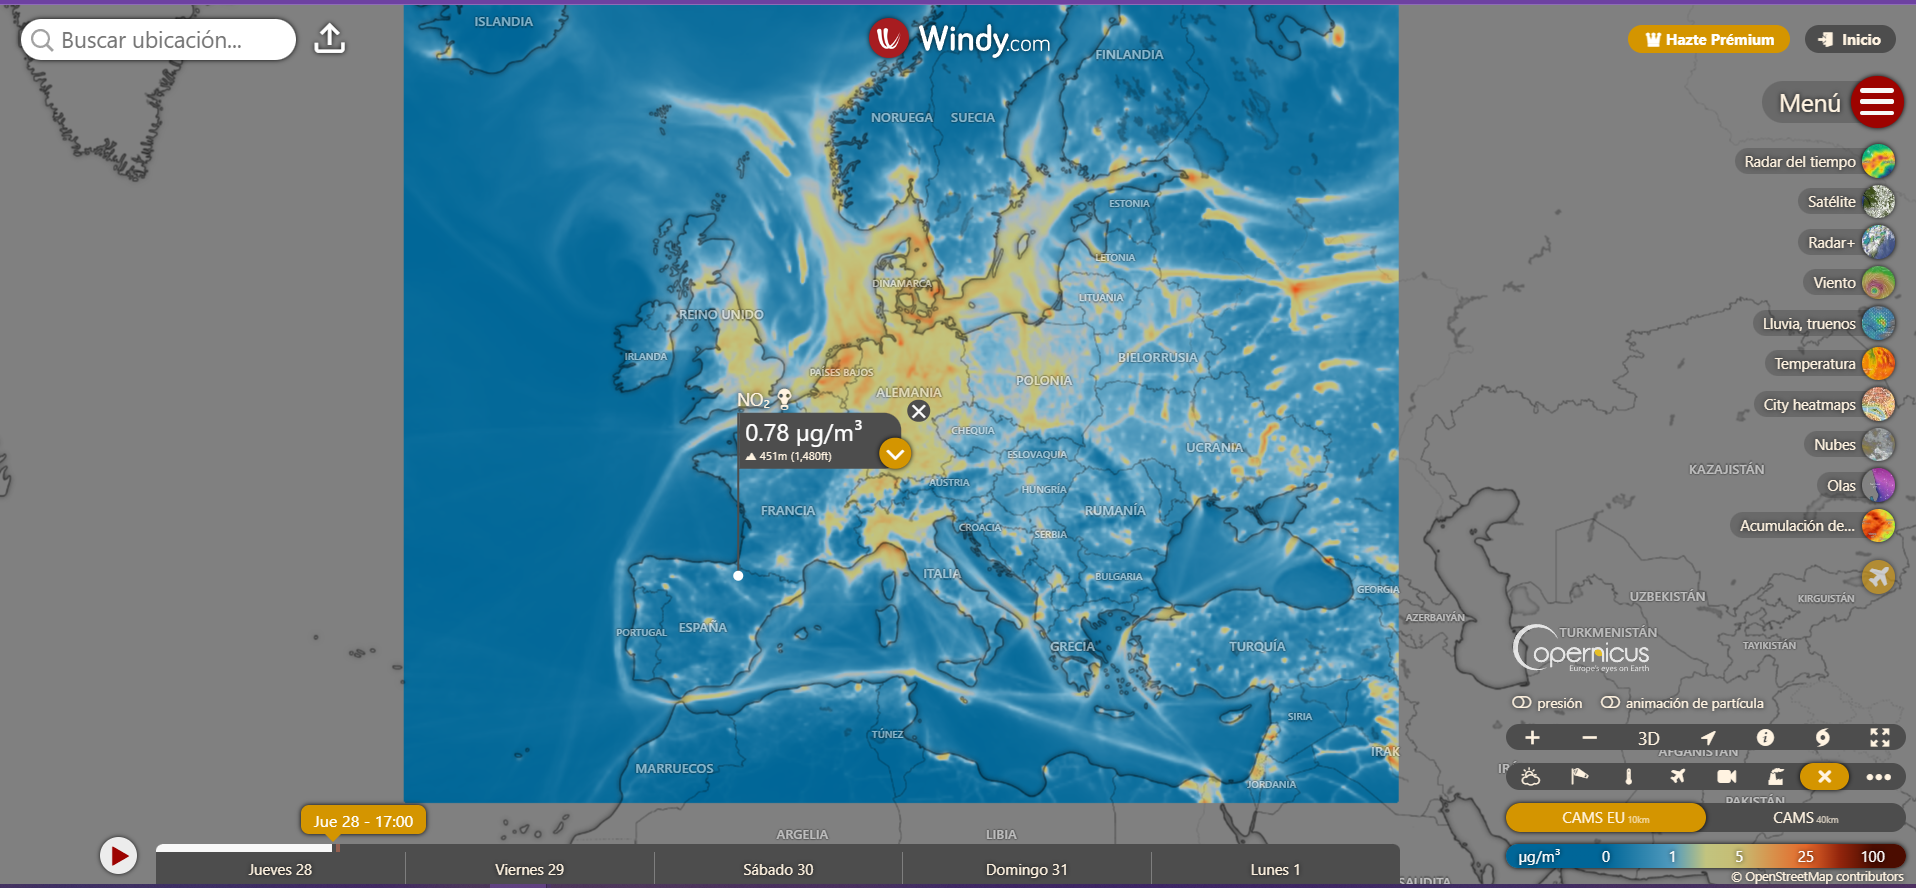
\includegraphics[width=0.75\textwidth]{fig/windy-example.png}
	\caption[Windy.com interface]{Example of CAMS air quality layers integrated in Windy.com.}
	\label{fig:windy}
\end{figure}

At the other end of the spectrum, the \textbf{CAMS Atmosphere Data Store (ADS)}\footnote{\href{https://ads.atmosphere.copernicus.eu/}{https://ads.atmosphere.copernicus.eu/}} provides full access to forecast datasets in scientific formats such as NetCDF and GRIB. Through ADS, expert users can download multi-day, hourly predictions of pollutants, meteorological variables, and greenhouse gases at global or regional scales. This platform offers maximum flexibility and scientific robustness, but requires specialized knowledge of data processing tools (Python, R, GIS software). For many non-experts, this represents a significant barrier. To illustrate, Figure~\ref{fig:ads} shows the ADS interface alongside a capture of the installation instructions for the CDS API, demonstrating the technical steps required to access the data programmatically.

\begin{figure}[h!btp]
	\centering
	
\includegraphics[width=0.75\textwidth]{fig/ads-example.png}
	\caption[CAMS Atmosphere Data Store]{Interface of the CAMS Atmosphere Data Store (ADS).}
	\label{fig:ads}
\end{figure}

\begin{figure}[h!btp]
	\centering
	
\includegraphics[width=0.75\textwidth]{fig/ads-example2.png}
	\caption[ADS API setup]{Screenshot illustrating the installation and setup of the CDS API for accessing ADS data.}
	\label{fig:ads2}
\end{figure}

Between these extremes, the \textbf{CAMS Regional Air Quality Viewer}\footnote{\href{https://atmosphere.copernicus.eu/european-air-quality-forecast-plots}{https://atmosphere.copernicus.eu/european-air-quality-forecast-plots}} is designed specifically to display European forecasts with higher spatial resolution (5–10 km). It presents interactive maps for pollutants such as ozone, nitrogen dioxide, and particulate matter. Unlike ADS, this platform allows users to visualize pollutant distributions graphically, including plots of predicted values over time. However, users cannot extract raw numerical data directly from the graphs, limiting its usefulness for advanced analysis (Figures~\ref{fig:regional-map} and \ref{fig:regional-graph}).

\begin{figure}[h!btp]
	\centering
	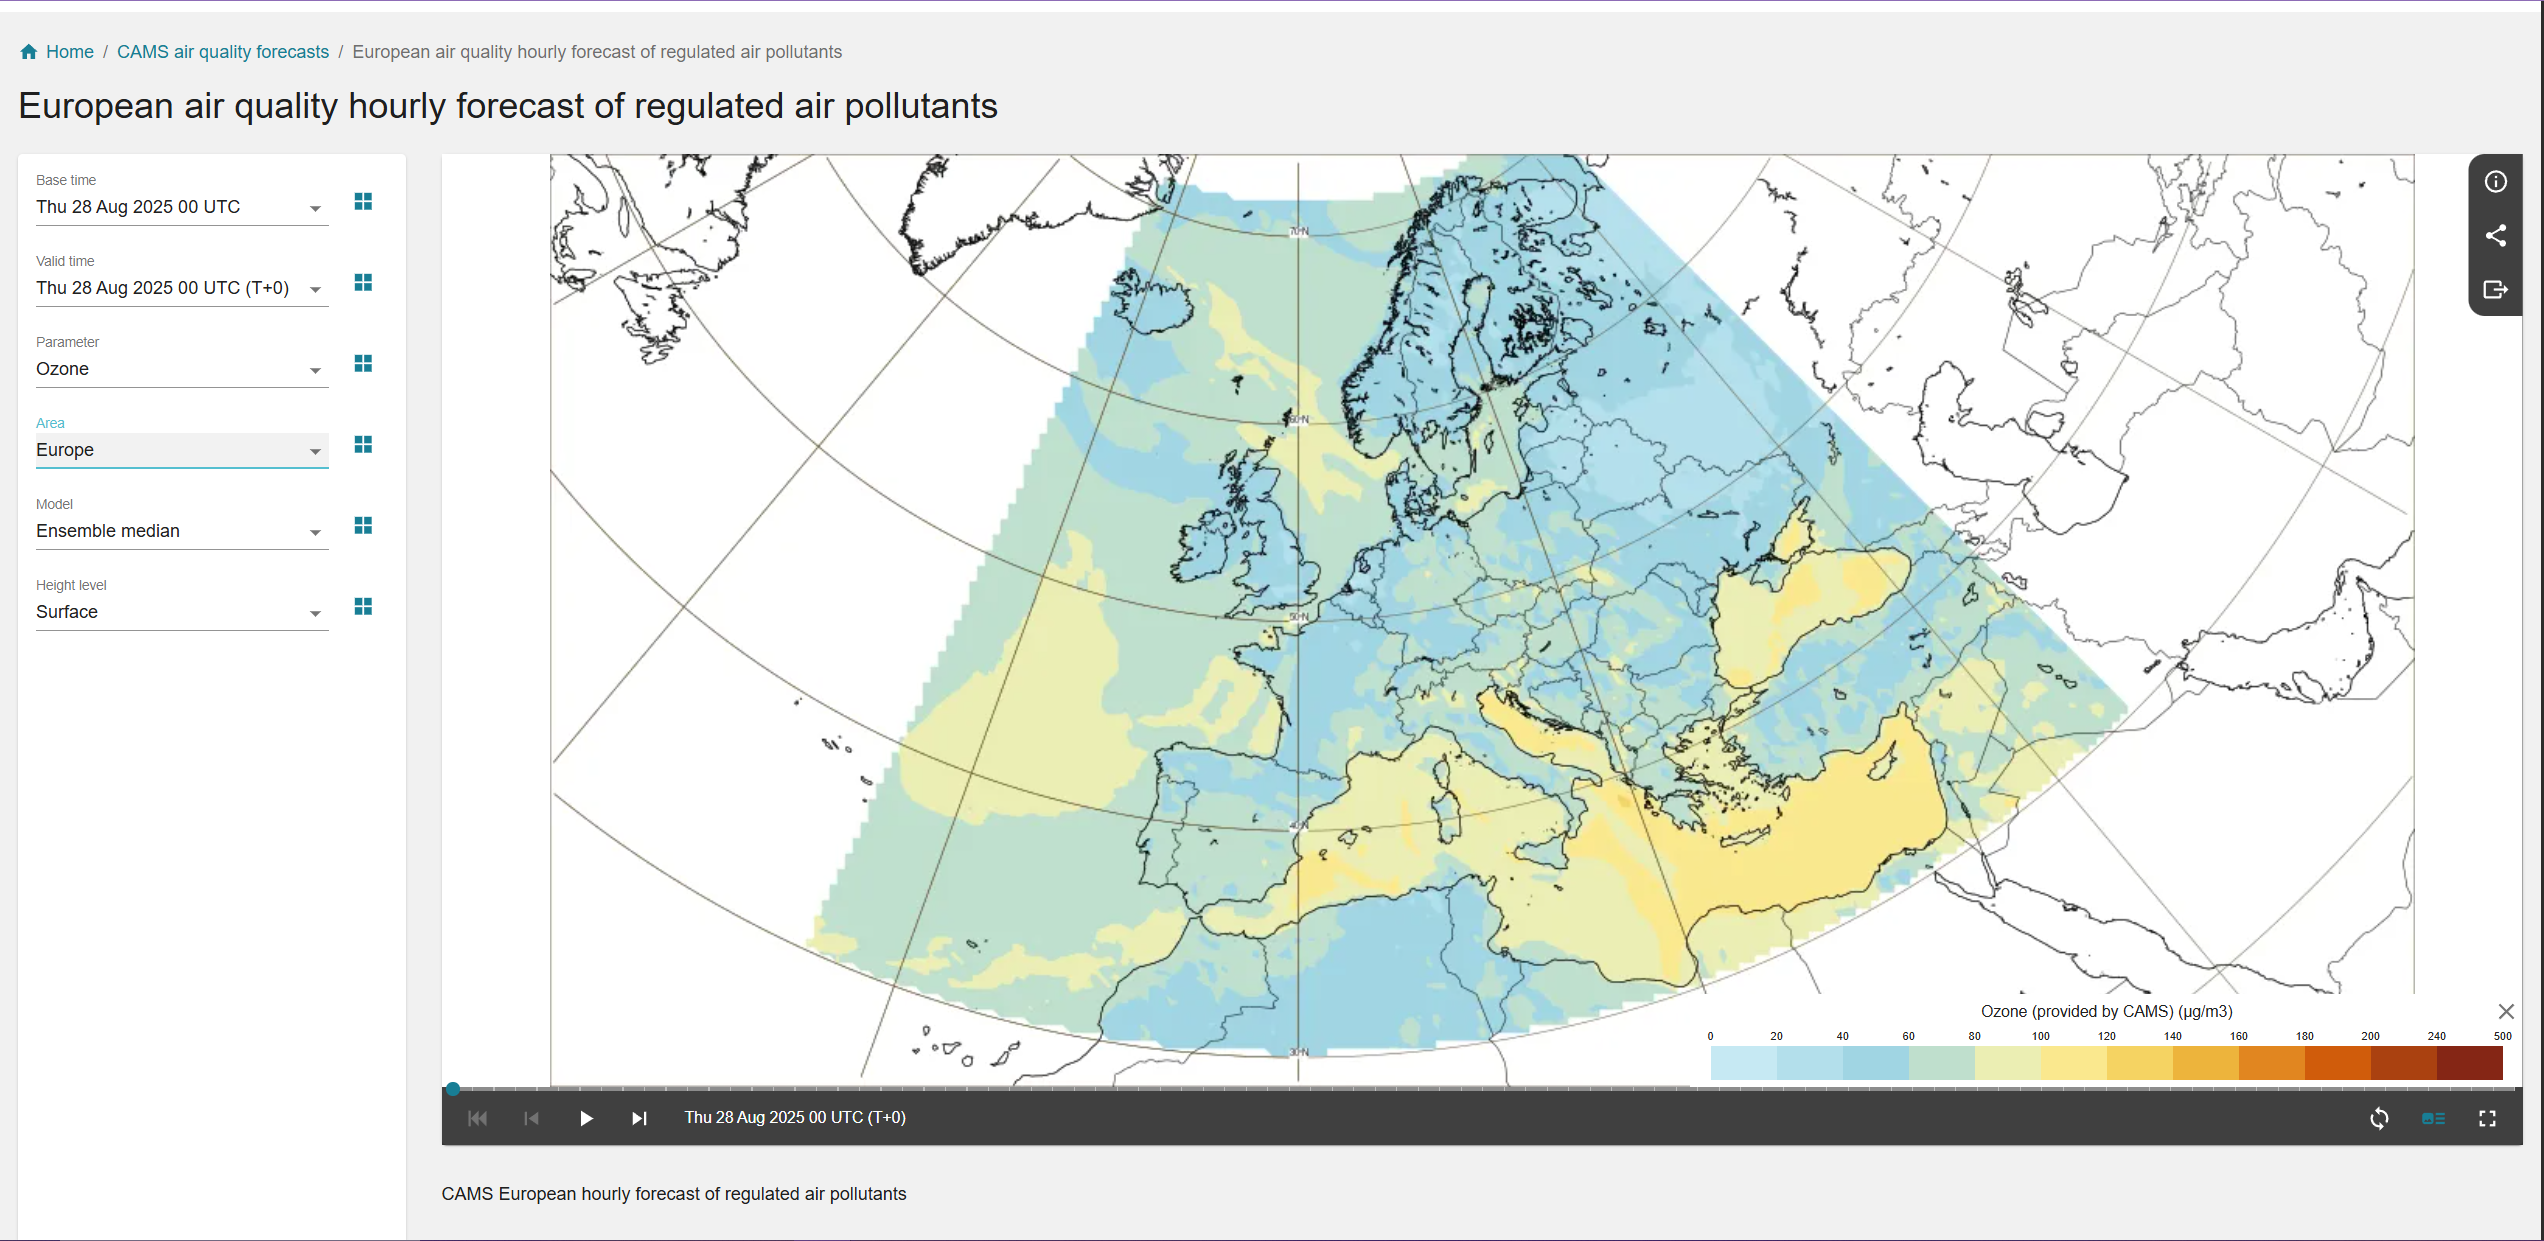
\includegraphics[width=0.75\textwidth]{fig/regional-example.png}
	\caption[CAMS Regional Viewer - Map]{CAMS Regional Air Quality Viewer, showing forecast maps for Europe.}
	\label{fig:regional-map}
\end{figure}

\begin{figure}[h!btp]
	\centering
	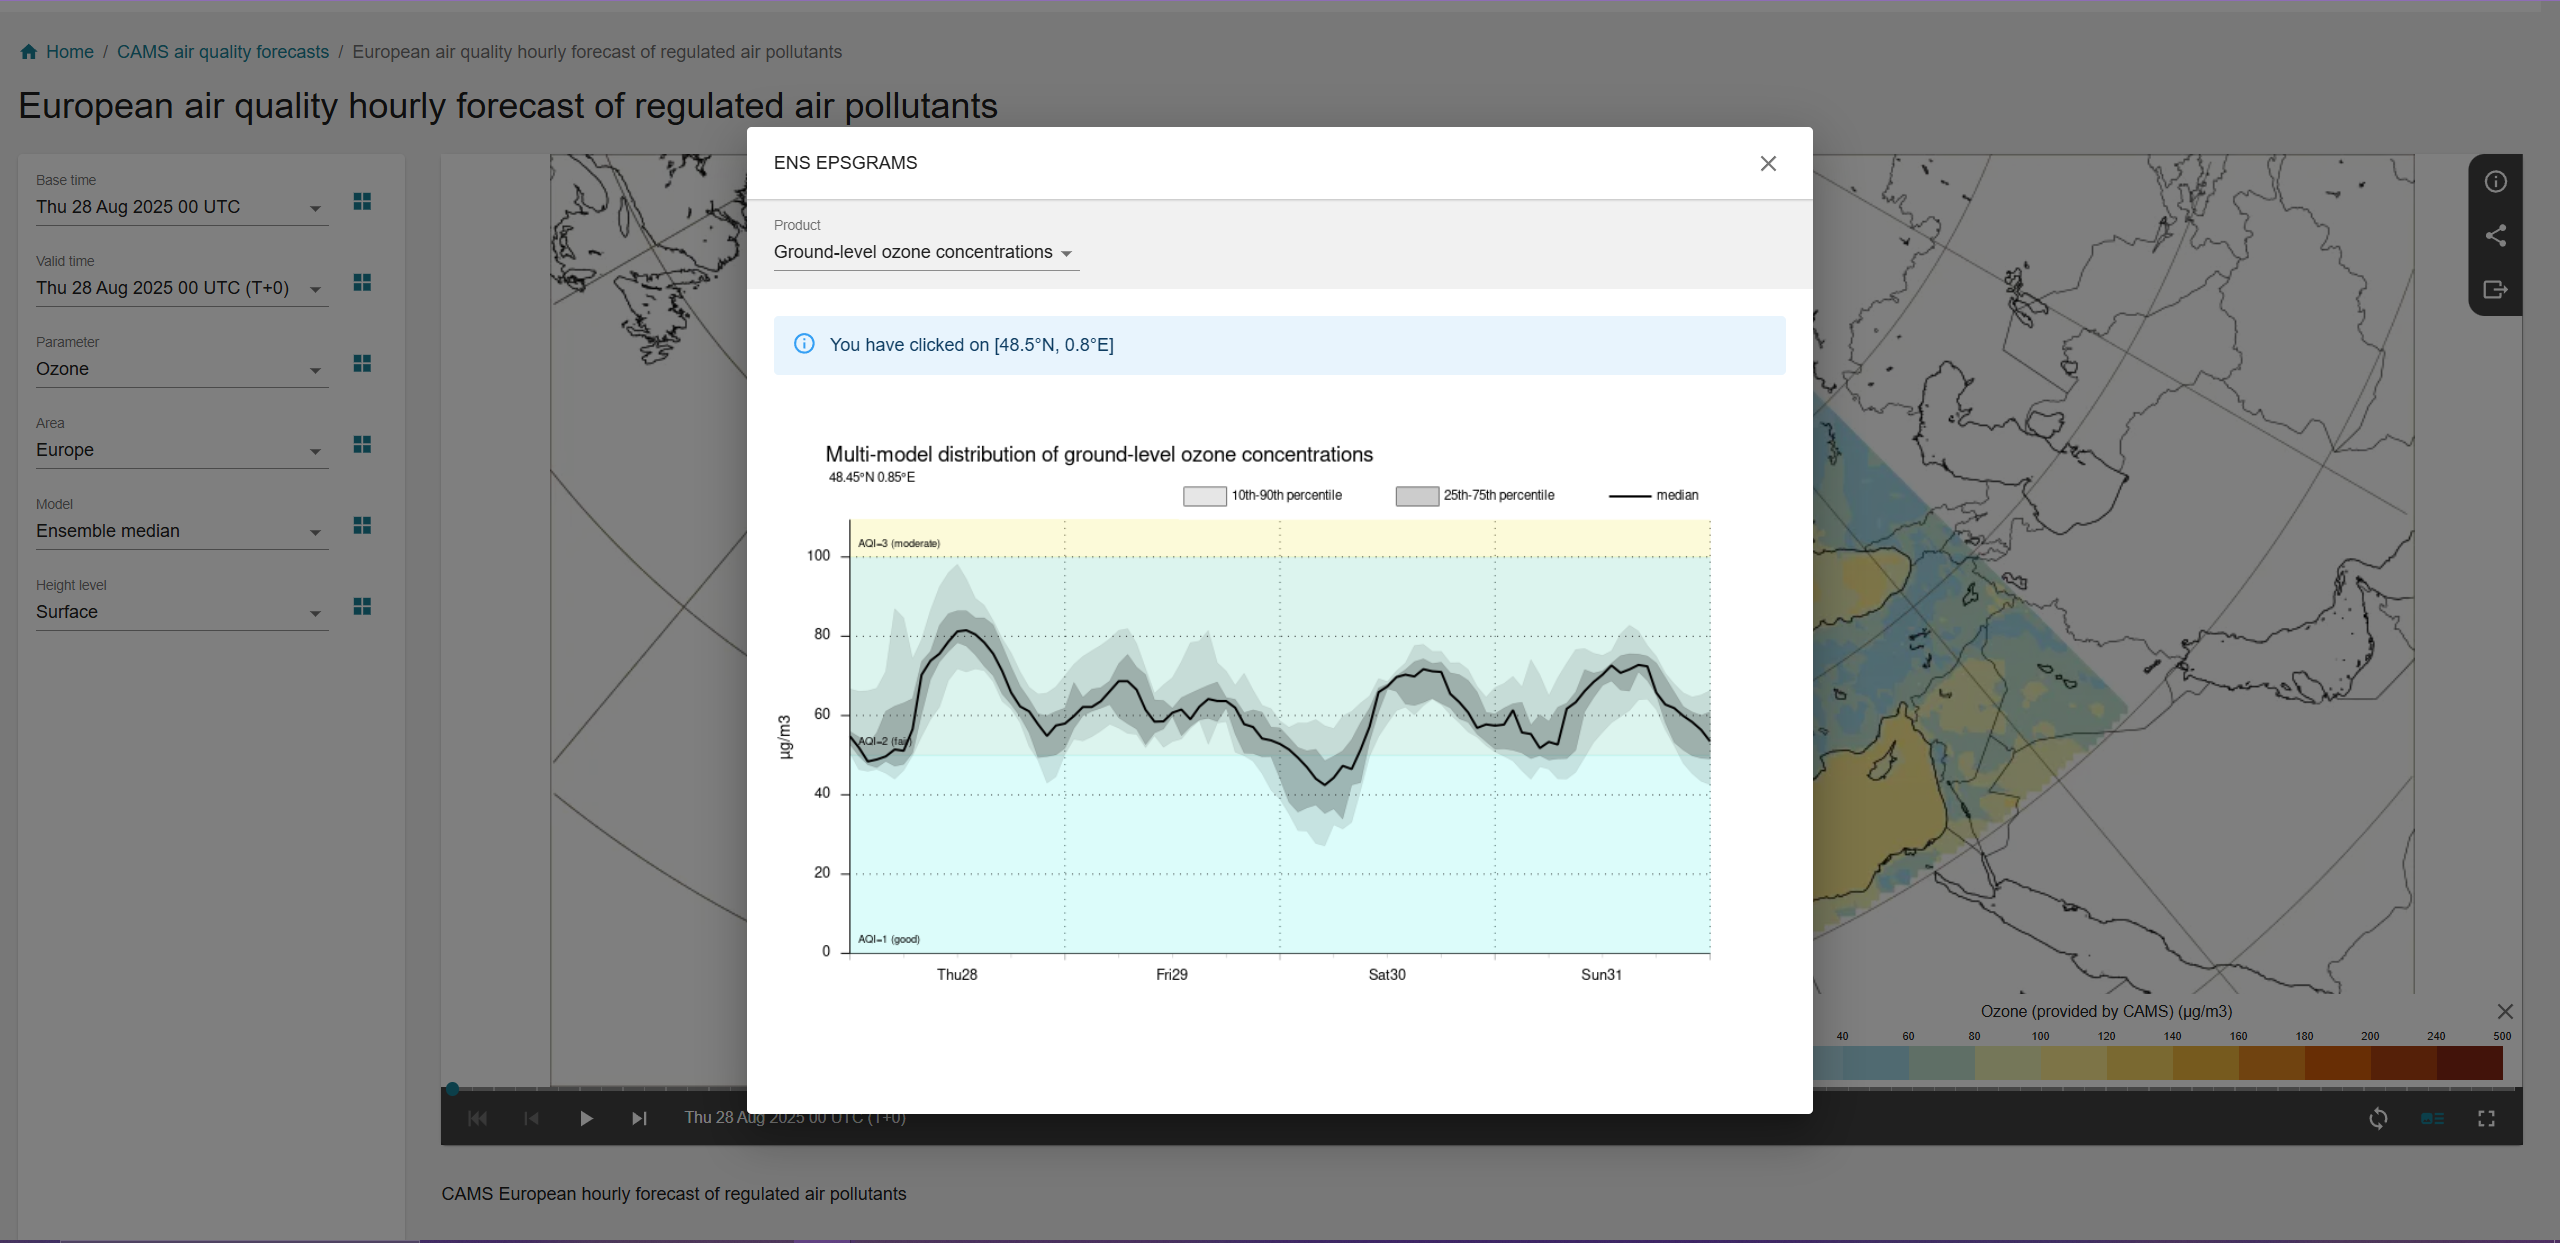
\includegraphics[width=0.75\textwidth]{fig/regional-example2.png}
	\caption[CAMS Regional Viewer - Graph]{Example of a graph in the CAMS Regional Air Quality Viewer, showing predicted pollutant values over time for a selected location.}
	\label{fig:regional-graph}
\end{figure}

In addition to forecast-oriented services, \textbf{OpenAQ} plays an important complementary role by aggregating real-time observational data from thousands of monitoring stations worldwide. Unlike CAMS platforms, OpenAQ focuses on measurements rather than modeled forecasts, making it particularly valuable for validation purposes. Researchers and developers can access its open API to retrieve raw observations, enabling integration into independent applications. While it does not provide predictive capability, OpenAQ exemplifies how open data platforms can foster transparency and community engagement.

In summary, existing platforms present a clear trade-off between usability and scientific depth. Public-facing tools like Windy.com offer engaging visualizations but little analytical flexibility, while scientific portals such as ADS provide full datasets at the expense of accessibility. Intermediate solutions, like the CAMS Regional Viewer, address part of this gap but remain limited in interactivity. This fragmentation highlights the need for tools that are at once scientifically robust and user-friendly, providing accessible, interactive ways to explore CAMS data without requiring advanced technical expertise.



\section{Challenges and Open Gaps}

I decided to develop my own platform for air quality forecasting because existing tools, although comprehensive, do not offer the flexibility needed to visualize information interactively and customize it according to specific regions and pollutants. Traditional platforms often provide static maps or pre-determined reports, whereas this application allows users to select different regions, choose specific pollutants, and observe their hourly variations through a slider, complemented by historical time-series charts. The integration of WMS layers and dynamic map visualization enables a more intuitive experience, allowing users to explore data in real time and obtain precise information by clicking on a given location. This approach contrasts with previous systems, which typically limit interactivity and do not allow combining visualizations from multiple sources dynamically. By developing this platform, the goal was to merge data accuracy with usability and analytical capability, resulting in a tool that is both accessible and versatile for public, academic, or environmental monitoring purposes.

Overall, existing tools successfully deliver high-quality air quality forecasts but exhibit trade-offs between usability and analytical depth. This motivates the creation of a new visualization platform that bridges this gap, offering a scientifically robust, interactive, and user-centered interface that facilitates exploration, comparison, and interpretation of atmospheric data.
